\documentclass[10pt,a4paper]{article}
\usepackage[a4paper, margin=2.1cm]{geometry}
\usepackage[T1]{fontenc}
\usepackage{lmodern}
\usepackage{microtype}
\usepackage{amsmath, amssymb}
\usepackage{booktabs, tabularx, multirow}
\usepackage{xcolor}
\usepackage{tikz}
\usetikzlibrary{arrows.meta, positioning, calc, decorations.pathreplacing}
\usepackage{pgfplots, pgfplotstable}
\usepgfplotslibrary{groupplots}
\usepackage{caption}
\usepackage{placeins}
\captionsetup{font=small, labelfont=bf}
\usepackage[hidelinks]{hyperref}
\usepackage[capitalise]{cleveref}
% Figure style: palette slots (validated categorical order, light mode), text inks and recessive axes.
\definecolor{sOne}{HTML}{2A78D6}    % series 1, blue
\definecolor{sTwo}{HTML}{EB6834}    % series 2, orange
\definecolor{sThree}{HTML}{1BAF7A}  % series 3, aqua
\definecolor{sFour}{HTML}{EDA100}   % series 4, yellow
\definecolor{sOther}{HTML}{A8A6A0}  % neutral "other"
\definecolor{inkOne}{HTML}{0B0B0B}
\definecolor{inkTwo}{HTML}{52514E}
\definecolor{gridc}{HTML}{E4E3DE}
\definecolor{boxfill}{HTML}{F4F3EF}

\pgfplotsset{
  compat=1.18,
  paper/.style={
    axis line style={draw=inkTwo, line width=0.4pt},
    tick style={draw=inkTwo, line width=0.4pt},
    major tick length=2pt,
    tick label style={font=\scriptsize, text=inkTwo},
    label style={font=\footnotesize, text=inkOne},
    title style={font=\footnotesize\bfseries, text=inkOne},
    legend style={font=\scriptsize, draw=none, fill=none, text=inkOne},
    legend cell align=left,
    grid style={draw=gridc, line width=0.4pt},
    every axis plot/.append style={line width=1pt},
  },
  dotfp/.style={only marks, mark=*, mark size=1.9pt, draw=white, line width=0.5pt, fill=sOne},
  dotag/.style={only marks, mark=diamond*, mark size=2.3pt, draw=white, line width=0.5pt, fill=sTwo},
}
\tikzset{
  box/.style={draw=inkTwo, line width=0.5pt, rounded corners=2pt, fill=boxfill, align=center, font=\footnotesize,
    inner sep=3pt},
  note/.style={font=\scriptsize, text=inkTwo, align=center},
  arr/.style={-{Stealth[length=4pt]}, draw=inkTwo, line width=0.6pt},
}

\usepackage{xspace}
\usepackage{url}
\makeatletter\g@addto@macro\UrlBreaks{\do\_}\makeatother
\urlstyle{tt}
\newcommand{\flag}[1]{\nolinkurl{#1}}
\newcommand{\ms}{\,ms\xspace}
\newcommand{\s}{\,s\xspace}
\emergencystretch=1.5em

\title{Communication and Runtime Engineering\\for Two-Party ResNet Inference in HPMPC\\[4pt]
\large ABY2 with HE and silent-OT preprocessing}
\author{Technical report, HPMPC \texttt{dbg} branch\\[2pt]
\small hpmpc \texttt{4dd999b}, ConvTriple \texttt{3e80748}, flexNN \texttt{ce50579}}
\date{September 29, 2026}

\begin{document}
\maketitle

\begin{abstract}
We describe the optimizations and fixes that make HPMPC's two-party ABY2 inference of ResNet50 fast,
reproducible and correct across all of its protocol variants. The work targets both communication and
runtime, in the preprocessing phase (homomorphic encryption for linear layers, silent OT for Boolean
material) and in the online phase (round latency and per-round work). For one ImageNet image,
preprocessing drops from 17.1\s to 4.3\s on two AMD EPYC 7543 hosts (3.2\s on EPYC 9354) and
its triple traffic from 1112 to 587\,MiB. The online phase drops from 2.4--4.3\s to 0.70\s.
BatchNorm triples shrink from 5.7\,GB to 0.19\,GB of traffic per
10 CIFAR-10 images, and Beaver 3- and 4-tuples need half the OTs and about 45\% less traffic.
On CIFAR-10 we evaluate 30 protocol variants (three MSB adders, five ReLU families, fused and unfused
BatchNorm) in single-batch and 192-image multi-batch mode on two machine pairs. Per 10 images, preprocessing takes 1.6--3.1\s and the online phase 0.35--0.52\s; 192 images take 12.5--24.4\s of preprocessing. With public weights, which need no linear-layer triples, preprocessing takes 0.9--2.0\s per 10 images.
With the AdamW-trained ResNet50, every variant classifies 62--73 of 100 images (plaintext 76) and
60--69\% of 192 images (plaintext 71.9\%). Along the way we fixed a thread race, two connection hangs, two protocol
bugs that broke whole variant families, and the sources of run-to-run nondeterminism: all 60
threaded builds now reproduce their serial reference bit for bit.
\end{abstract}

\section{Introduction}

Two-party inference with a preprocessing phase splits the cost of a secure neural network into two
parts. An input-independent \emph{preprocessing phase} produces correlated randomness: multiplication
triples for the linear layers, generated with homomorphic encryption (HE), and Boolean triples and
tuples for the nonlinear layers, generated with oblivious transfer (OT). The \emph{online phase} then
evaluates the network on masked values and needs only a few messages per layer. HPMPC implements this
design with an ABY2-style protocol~\cite{aby2} (\flag{PROTOCOL=4}) and generates its preprocessing
material with the CHEETAH~\cite{cheetah} HE and silent-OT~\cite{ferret} machinery (ConvTriple).

This report collects the engineering work that took this pipeline from a working prototype to a fast
and reproducible system. Its focus is communication and runtime; \cref{fig:summary} summarizes the largest effects.

\begin{itemize}\itemsep1pt
\item \textbf{HE preprocessing} (\cref{sec:he}): a packed and pipelined convolution evaluator, an exact
  wire format that sends only the bits decryption needs, and BatchNorm triples packed into full
  ciphertexts and generated for all layers in one product. ImageNet preprocessing: $17.1\s \to 4.3\s$ ($4.0\times$).
\item \textbf{Boolean preprocessing} (\cref{sec:ot}): OT packs sized by total demand, ferret parameters and
  a prefetching LPN step, \flag{TCP_NODELAY} on every channel, bit-packed random OTs, and Beaver tuples
  whose products share one OT per common factor (half the OTs, ${\approx}45\%$ less traffic).
\item \textbf{Online phase} (\cref{sec:online}): Nagle-free sockets, element-parallel circuit levels for
  batch size one, pooled GEMM threads, an ahead-of-time PRNG and fewer rounds per ReLU. ImageNet online: $2.4\text{--}4.3\s \to 0.70\s$.
\item \textbf{Correctness and reproducibility} (\cref{sec:correct}): deterministic OT and HE randomness,
  and fixes for a worker race, lost wake-ups, stale listeners, multi-batch A2B and public-weight BatchNorm.
\item \textbf{Evaluation} (\cref{sec:eval}): 30 variants $\times$ 2 batch modes $\times$ 2 machine pairs,
  with final accuracy on a trained model.
\end{itemize}

\begin{figure}[t]
  \centering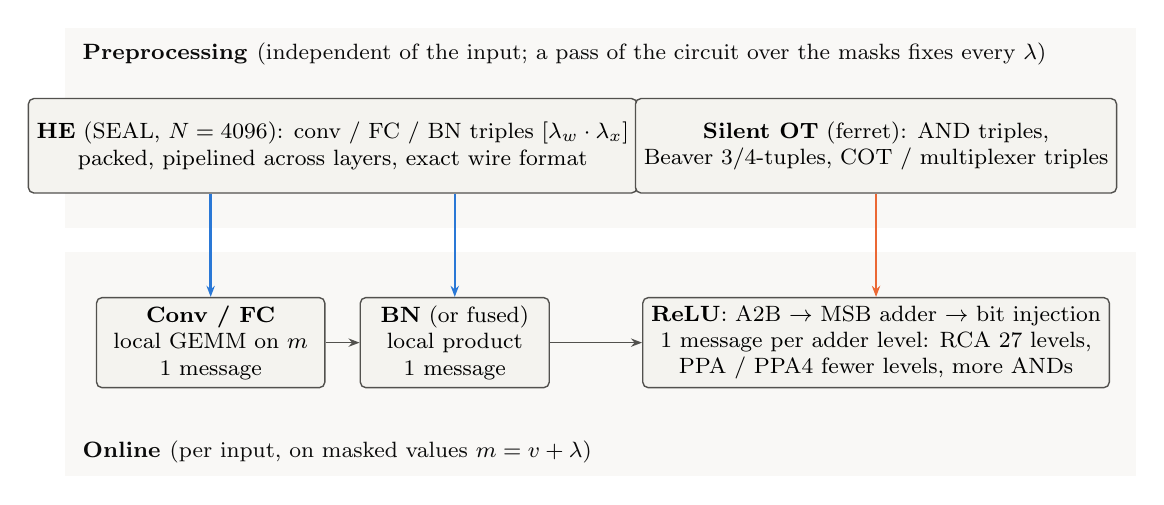
\begin{tikzpicture}
  % bands
  \fill[boxfill!55] (-0.2,0.25) rectangle (13.4,-2.3);
  \fill[boxfill!55] (-0.2,-2.6) rectangle (13.4,-5.45);
  \node[anchor=north west, font=\footnotesize\bfseries, text=inkOne] at (-0.1,0.18)
    {Preprocessing \textmd{(independent of the input; a pass of the circuit over the masks fixes every $\lambda$)}};
  \node[anchor=south west, font=\footnotesize\bfseries, text=inkOne] at (-0.1,-5.4)
    {Online \textmd{(per input, on masked values $m = v + \lambda$)}};

  % preprocessing sources, each above the layers that consume it
  \node[box, minimum width=5.9cm, minimum height=1.2cm] (he) at (3.2,-1.25)
    {\textbf{HE} (SEAL, $N = 4096$): conv / FC / BN triples $[\lambda_w\cdot\lambda_x]$\\
     packed, pipelined across layers, exact wire format};
  \node[box, minimum width=5.8cm, minimum height=1.2cm] (ot) at (10.1,-1.25)
    {\textbf{Silent OT} (ferret): AND triples,\\Beaver 3/4-tuples, COT / multiplexer triples};

  % online chain
  \node[box, minimum width=2.9cm, minimum height=1.1cm] (conv) at (1.65,-3.75)
    {\textbf{Conv / FC}\\local GEMM on $m$\\1 message};
  \node[box, minimum width=2.4cm, minimum height=1.1cm] (bn) at (4.75,-3.75)
    {\textbf{BN} (or fused)\\local product\\1 message};
  \node[box, minimum width=5.8cm, minimum height=1.1cm] (relu) at (10.1,-3.75)
    {\textbf{ReLU}: A2B $\rightarrow$ MSB adder $\rightarrow$ bit injection\\
     1 message per adder level: RCA 27 levels,\\PPA / PPA4 fewer levels, more ANDs};
  \draw[arr] (conv) -- (bn);
  \draw[arr] (bn) -- (relu);

  \draw[arr, draw=sOne, line width=0.9pt] (conv.north |- he.south) -- (conv.north);
  \draw[arr, draw=sOne, line width=0.9pt] (bn.north |- he.south) -- (bn.north);
  \draw[arr, draw=sTwo, line width=0.9pt] (ot.south) -- (relu.north);
\end{tikzpicture}

  \caption{Where the cost of 2PC inference arises. A preprocessing pass fixes every mask; HE produces the
  linear-layer triples and silent OT the Boolean material. Online, a linear layer costs one message and a
  ReLU one message per level of its MSB adder.}
  \label{fig:overview}
\end{figure}

\begin{figure}[t]
  \centering% Headline effects: traffic reductions (left) and runtime speedups (right), each labeled before -> after.
\pgfplotstableread{
i red txt label
0 96.7 {5733 $\to$ 187 MB} {BN triples, 10 CIFAR images}
1 47.2 {1112 $\to$ 587 MiB} {all triples, 1 ImageNet image}
2 46.4 {40.2 $\to$ 21.5 MB} {Beaver 3-tuples, per process}
3 43.4 {66.7 $\to$ 37.8 MB} {Beaver 4-tuples, per process}
4 18.5 {588 $\to$ 479 MiB} {conv triples, exact wire format}
5 61.6 {7188 $\to$ 2763 MB} {multi-batch preprocessing, 192 images}
6 10.7 {23.3 $\to$ 20.8 MB} {ReLU online traffic, RCA (CUT)}
}\traffic
\pgfplotstableread{
i speed txt label
0 32.6 {6.2 $\to$ 0.19 s} {BN triples, 10 CIFAR images}
1 7.4 {12.9 $\to$ 1.7 s} {conv triples, 1 ImageNet image}
2 4.0 {17.1 $\to$ 4.3 s} {preprocessing, 1 ImageNet image}
3 3.5 {2.4 $\to$ 0.70 s} {online, 1 ImageNet image}
4 2.4 {8.4 $\to$ 3.5 s} {PPA a2b preprocessing (Nagle off)}
5 2.1 {19.0 $\to$ 9.2 s} {Beaver tuples, per process}
6 2.2 {8.6 $\to$ 3.9 s} {multi-batch conv triples, per process}
7 2.0 {0.36 $\to$ 0.18 s} {conv triples, CIFAR (concurrent AB2)}
8 1.8 {25.0 $\to$ 14.0 s} {multi-batch HE/OT threads}
}\speed
\begin{tikzpicture}
\begin{axis}[
  paper, name=traffic, width=8.2cm, height=5.4cm, y dir=reverse, ymin=-0.6, ymax=6.6,
  xbar, bar width=7pt, xmin=0, xmax=100, xlabel={less traffic (\%)},
  ytick=data, yticklabels from table={\traffic}{label}, xmajorgrids, axis x line*=bottom, axis y line*=left,
  title={Communication},
  nodes near coords, point meta=explicit symbolic,
  every node near coord/.style={font=\scriptsize, text=inkTwo, anchor=west, xshift=1pt},
]
  \addplot[fill=sOne, draw=none] table[x=red, y=i, meta=txt] {\traffic};
\end{axis}
\begin{axis}[
  paper, at={(traffic.south west)}, anchor=north west, yshift=-1.75cm, width=8.2cm, height=6.6cm, y dir=reverse,
  ymin=-0.6, ymax=8.6, xbar, bar width=7pt, xmode=log, xmin=1, xmax=100, log basis x=10,
  xtick={1,2,5,10,20,50,100}, xticklabels={1$\times$,2$\times$,5$\times$,10$\times$,20$\times$,50$\times$,100$\times$},
  xlabel={speedup}, ytick=data, yticklabels from table={\speed}{label}, xmajorgrids,
  axis x line*=bottom, axis y line*=left, title={Runtime},
  nodes near coords, point meta=explicit symbolic,
  every node near coord/.style={font=\scriptsize, text=inkTwo, anchor=west, xshift=1pt},
]
  \addplot[fill=sTwo, draw=none] table[x=speed, y=i, meta=txt] {\speed};
\end{axis}
\end{tikzpicture}

  \caption{Headline effects of the changes in this report, each labeled with its before and after values. Communication:
  share of traffic removed. Runtime: speedup (log scale). Sections~\ref{sec:he}--\ref{sec:multi} explain each.}
  \label{fig:summary}
\end{figure}

\section{Setting}\label{sec:setting}

\paragraph{Protocol.} ABY2 shares a value $v$ as a public masked value $m = v + \lambda$ together with
additive shares of the mask $\lambda = \lambda_0 + \lambda_1$. Every mask is fixed in preprocessing, so a
linear layer is local except for one message that re-masks its output, and its preprocessing is a triple
over the masks, e.g.\ $[\lambda_w \cdot \lambda_x]$ for a convolution (\cref{fig:overview}). With
\flag{A_KNOWN=1} the model owner P0 holds the weight masks and the data owner P1 the activation masks
(the AB2 triple); with \flag{A_KNOWN=0} both are shared (AB). A ReLU converts its input to Boolean
shares (A2B), extracts the sign with an MSB adder and injects the bit back into the arithmetic domain
(bit injection). The adder sets the number of online rounds per ReLU: the ripple-carry adder
(RCA) needs 27 AND levels, the parallel-prefix adders PPA and PPA4 (4-input prefix gates, which use
Beaver 3- and 4-tuples) need fewer levels but more AND gates.

\paragraph{Variants.} We measure three adders (RCA, PPA, PPA4) and five ReLU families: \emph{plain};
\emph{reshare} (\flag{RESHARE_OPT}); \emph{reshare+sim}, which folds the reshare material into the
convolution mask (\flag{RESHARE_OPT_SIM}); \emph{a2b}, which moves the A2B to preprocessing and bakes its
mask into the convolution output (\flag{A2B_ONLINE_OPT}, \flag{A2B_CONV_BAKE}); and \emph{a2b+AKTE}, an
adder for inputs whose mask the evaluators know (\flag{A_KNOWN_TO_EVALUATORS_OPT}). Each variant runs with
BatchNorm fused into the preceding convolution or unfused. All variants share \flag{BITLENGTH=32},
\flag{FRACTIONAL=5}, probabilistic (SecureML-style) truncation, \flag{FUSE_RELU_AVG=1} and
\flag{CUT_FRACTIONAL_BITS_OPT=1}.

\paragraph{Workloads.} ResNet50 on CIFAR-10 in two modes. \emph{Single batch}: one process,
32-bit lanes (\flag{DATTYPE=32}), 10 images, 32 HE/OT threads and 31 extra online threads.
\emph{Multi-batch}: 24 processes with 256-bit registers of eight 32-bit lanes, 192 images, 3 HE/OT
threads and one extra online thread per process. The HE preprocessing study uses ResNet50 on one
$224\times224$ ImageNet image.

\begin{table}[t]
\centering\small
\begin{tabularx}{\linewidth}{@{}lXX@{}}
\toprule
& flare / polynize & algofi / goracle \\
\midrule
CPU & AMD EPYC 9354 (Zen 4), AVX-512, VAES, IFMA & AMD EPYC 7543 (Zen 3), AVX2, AES-NI \\
Cores, memory & 32 cores / 64 threads, 752\,GB & 32 cores / 64 threads, 512\,GB \\
Link & \multicolumn{2}{l}{25\,Gbit/s direct (Intel E810, ice 2.6.7), MTU 9700, 24.7\,Gbit/s iperf3, RTT 0.28--0.31\ms} \\
Roles & \multicolumn{2}{l}{P0 (model owner): flare / algofi; P1 (data owner): polynize / goracle} \\
\bottomrule
\end{tabularx}
\caption{Machines. Each host builds its own binaries (\texttt{-march=native}).}
\label{tab:machines}
\end{table}

\paragraph{Measurement.} Preprocessing and online time are P0's wall-clock times (the maximum over
processes in multi-batch). Single-batch numbers are medians of two runs; multi-batch runs once.
All randomness is seeded, so every run of a build produces a
bit-identical output; we check each run's output hash against a serial build without extra threads
(\cref{sec:correct}). The runtime does not depend on the weights: HE triples are generated with
\flag{TRIPLE_ZERO=ON} and no code path skips zero values.
Accuracy uses two trained ResNet50 models: \texttt{Cifar\_adam\_001} for the runtime matrix and an
AdamW-trained model (74.35\% on the test set) for the final accuracy.

% ------------------------------------------------------------------------------------------------
\section{Linear layers: HE preprocessing}\label{sec:he}

\Cref{fig:steps} traces ImageNet preprocessing through the ten ConvTriple changes (s1--s10); \cref{tab:steps} lists what each step does.

\begin{figure}[t]
  \centering\begin{tikzpicture}
\begin{groupplot}[
  group style={group size=1 by 2, vertical sep=6mm, xticklabels at=edge bottom},
  paper, width=0.98\linewidth, xmin=-0.6, xmax=10.6,
  xtick={0,...,10}, xticklabels from table={data/imagenet_steps.dat}{step},
  ymajorgrids, axis x line*=bottom, axis y line*=left,
]
\nextgroupplot[
  height=6.2cm, ybar stacked, bar width=13pt, ymin=0, ymax=19.5,
  ylabel={preprocessing (s)},
  legend style={at={(0.99,0.98)}, anchor=north east, legend columns=1},
  reverse legend,
]
  \addplot[fill=sOne, draw=white, line width=0.8pt] table[x=x, y=conv] {data/imagenet_steps.dat};
  \addplot[fill=sTwo, draw=white, line width=0.8pt] table[x=x, y=keysetup] {data/imagenet_steps.dat};
  \addplot[fill=sThree, draw=white, line width=0.8pt] table[x=x, y=bool] {data/imagenet_steps.dat};
  \addplot[fill=sFour, draw=white, line width=0.8pt] table[x=x, y=muxcotfc] {data/imagenet_steps.dat};
  \addplot[fill=sOther, draw=white, line width=0.8pt] table[x=x, y=other] {data/imagenet_steps.dat};
  \legend{conv triples (HE), key + OT setup, AND triples, MUX + COT + FC, other}
  % totals above the stacks
  \addplot[forget plot, ybar=0pt, draw=none, fill=none, nodes near coords, point meta=explicit symbolic,
    every node near coord/.style={font=\scriptsize, text=inkOne, anchor=south}]
    table[x=x, y expr=0.0001, meta=total] {data/imagenet_steps.dat};
\nextgroupplot[
  height=3.4cm, ybar, bar width=13pt, ymin=0, ymax=1300,
  ylabel={triples (MiB)},
  nodes near coords, every node near coord/.style={font=\scriptsize, text=inkTwo, anchor=south},
]
  \addplot[fill=inkTwo!55, draw=white] table[x=x, y=trafficMiB] {data/imagenet_steps.dat};
\end{groupplot}
\end{tikzpicture}

  \caption{Preprocessing of one ImageNet image on algofi / goracle, by component (median of 3 runs), and
  the triple traffic sent plus received by P0. s2--s6 are value-independent reruns (\cref{sec:zero}).}
  \label{fig:steps}
\end{figure}

\begin{table}[t]
\centering\small
\begin{tabularx}{\linewidth}{@{}lXrr@{}}
\toprule
Step & Change & Pre (s) & Conv (s)\\
\midrule
s0 & Baseline: CHEETAH's \texttt{HomConv2DSS}, one output ciphertext per channel and tile & 17.14 & 12.86\\
s1 & Packed layout: several images and output channels per ciphertext (traffic $1112\to698$\,MiB) & 17.95 & 13.65\\
s2 & Packed evaluator: weight polynomials transformed right before use, $1\times1$ weights through NTTs of size $N/2^a$, sparse polynomials from a power table, lazy 128-bit accumulation & 11.92 & 7.49\\
s3 & AES-CTR noise and masks instead of Blake2; ciphertexts loaded in parallel & 9.13 & 4.66\\
s4 & AND triples from bit-packed random OTs (64 per word) & 8.91 & 4.66\\
s5 & Thread pool kept across calls; multiply-accumulate blocked per prime & 7.00 & 2.82\\
s6 & Multiplexer and COT triples on all threads (MUX $1.08\to0.07\s$, COT $0.48\to0.04\s$) & 5.38 & 2.74\\
s7 & All work independent of the weights' values (\flag{TRIPLE_ZERO=ON}) & 5.37 & 2.62\\
s8 & Convolutions pipelined across layers (\cref{fig:pipeline}) & 4.66 & 1.90\\
s9 & Exact wire format and byte-optimal tiling (conv traffic $588\to479$\,MiB) & 4.45 & 1.71\\
s10 & Prefetching LPN step, ferret parameters b12 (key setup $1.42\to1.13\s$) & 4.26 & 1.74\\
\bottomrule
\end{tabularx}
\caption{The HE and OT preprocessing steps (ImageNet, algofi / goracle, 32 threads). The same build
preprocesses in 3.2--3.3\s on flare / polynize.}
\label{tab:steps}
\end{table}

\paragraph{Packed evaluator (s1, s2).} CHEETAH's convolution encrypts one input tile per ciphertext and
returns one ciphertext per output channel and tile. The packed layout of the GPU path puts several images
and output channels into each ciphertext: triple traffic falls from 1112 to 698\,MiB. At first this made the evaluator
slower (s1), because every weight polynomial still took a full NTT. The evaluator now transforms a weight
polynomial right before its only use, and it transforms $1\times1$ weights with NTTs of size
$N/2^a$. It builds sparse polynomials from a table of powers and sums products lazily in 128 bits.
Convolution time falls from 13.7 to 7.5\s.

\paragraph{Randomness and threads (s3--s6).} Flooding noise and masks come from an AES-CTR generator
(AES-NI) instead of SEAL's Blake2; the thread pool survives across the several parallel calls of a layer;
the multiplexer and COT triples run on all threads. Together these steps take preprocessing from 11.9 to 5.4\s.

\begin{figure}[t]
  \centering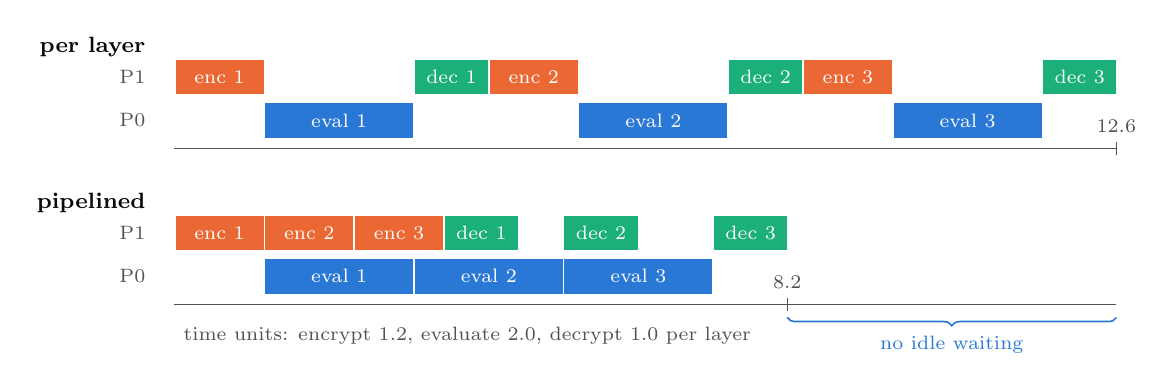
\begin{tikzpicture}[x=0.95cm, y=0.55cm]
  \tikzset{blk/.style={draw=white, line width=0.6pt, minimum height=0.46cm, inner sep=0pt, font=\scriptsize,
    text=white, anchor=west}}
  % \blk{start}{length}{row y}{color}{label}
  \newcommand{\blk}[5]{\node[blk, fill=#4, minimum width=#2*0.95cm] at (#1,#3) {#5};}
  % ---- per layer: enc (1.2) -> eval (2.0) -> dec (1.0), layer by layer
  \node[anchor=east, font=\footnotesize\bfseries, text=inkOne] at (-0.25,1.7) {per layer};
  \node[anchor=east, note] at (-0.25,1) {P1}; \node[anchor=east, note] at (-0.25,0) {P0};
  \foreach \l/\t in {1/0, 2/4.2, 3/8.4} {
    \blk{\t}{1.2}{1}{sTwo}{enc \l}
    \blk{\t+1.2}{2}{0}{sOne}{eval \l}
    \blk{\t+3.2}{1.0}{1}{sThree}{dec \l}
  }
  \draw[inkTwo, line width=0.4pt] (0,-0.65) -- (12.6,-0.65);
  \draw[inkTwo, line width=0.4pt] (12.6,-0.8) -- (12.6,-0.5) node[note, above] {12.6};
  % ---- pipelined: P1 encrypts ahead and decrypts behind while P0 evaluates
  \node[anchor=east, font=\footnotesize\bfseries, text=inkOne] at (-0.25,-1.9) {pipelined};
  \node[anchor=east, note] at (-0.25,-2.6) {P1}; \node[anchor=east, note] at (-0.25,-3.6) {P0};
  \blk{0}{1.2}{-2.6}{sTwo}{enc 1}
  \blk{1.2}{1.2}{-2.6}{sTwo}{enc 2}
  \blk{2.4}{1.2}{-2.6}{sTwo}{enc 3}
  \blk{3.6}{1.0}{-2.6}{sThree}{dec 1}
  \blk{5.2}{1.0}{-2.6}{sThree}{dec 2}
  \blk{7.2}{1.0}{-2.6}{sThree}{dec 3}
  \blk{1.2}{2}{-3.6}{sOne}{eval 1}
  \blk{3.2}{2}{-3.6}{sOne}{eval 2}
  \blk{5.2}{2}{-3.6}{sOne}{eval 3}
  \draw[inkTwo, line width=0.4pt] (0,-4.25) -- (12.6,-4.25);
  \draw[inkTwo, line width=0.4pt] (8.2,-4.4) -- (8.2,-4.1) node[note, above] {8.2};
  \draw[decorate, decoration={brace, amplitude=3pt, mirror}, draw=sOne, line width=0.6pt] (8.2,-4.55) -- (12.6,-4.55);
  \node[note, text=sOne, anchor=north] at (10.4,-4.75) {no idle waiting};
  \node[note, anchor=north west] at (0,-4.55) {time units: encrypt 1.2, evaluate 2.0, decrypt 1.0 per layer};
\end{tikzpicture}

  \caption{Pipelining the convolutions across layers (s8). Per layer, P1 waits while P0 evaluates and
  vice versa; pipelined, P1 encrypts the next layer's inputs and decrypts the previous layer's outputs
  while P0 evaluates. Same bytes, preprocessing $5.69\to4.66\s$.}
  \label{fig:pipeline}
\end{figure}

\paragraph{Pipelining (s8).} Per layer, each party idled while the other worked: at s7 P0 waited
0.82\s and P1 1.95\s in total. The pipelined protocol (\cref{fig:pipeline}) overlaps P1's
encryption and decryption with P0's evaluation. It sends exactly the same bytes and cuts convolution
time from 2.6 to 1.9\s; with \flag{A_KNOWN=0}, where both parties encrypt, from 3.9--4.0 to 2.0\s in
isolation.

\paragraph{Exact wire format (s9).} SEAL serializes a seeded input ciphertext with zstd to 62.4\,KB. P1
now sends only a 16-byte seed and $c_0$ at exactly $60+49=109$ bits per coefficient (55.8\,KB). P0
expands $c_1$ from the seed directly in NTT form, which saves an inverse and a forward NTT per input. For
outputs, the modulus switch before decryption keeps 34 bits of $c_0$ and 46 of $c_1$; exactly those bits
travel, 20--25\% less than zstd. The tile search now minimizes bytes rather than ciphertexts, since an
input costs about 2.4 times an output. Convolution traffic falls 18\% and all preprocessing traffic 12\%
(\cref{tab:traffic}); decrypted values are bit-identical, and a check rejects outputs whose dropped bits are
not zero. The 109-bit input modulus is a floor: BFV's plaintext product carries a term of up to
${\approx}2^{74}$.

\begin{table}[t]
\centering\small
\begin{tabular}{@{}lrr@{}}
\toprule
MiB, P0 sent / received & before (s8) & after (s10)\\
\midrule
Conv triples & 232.6 / 355.1 & 234.9 / 244.1\\
Ferret setup & 46.2 / 46.2 & 52.7 / 52.7\\
Multiplexer triples & 35.4 / 35.4 & 35.4 / 35.4\\
COT triples & 34.4 / 1.1 & 34.4 / 1.1\\
FC triples & 0.7 / 1.2 & 0.7 / 1.2\\
\midrule
Total & 349.4 / 439.0 (788.4) & 358.2 / 334.6 (692.8)\\
\bottomrule
\end{tabular}
\caption{Traffic of one ImageNet preprocessing (\flag{A_KNOWN=1}). With \flag{A_KNOWN=0} the triple
traffic falls from 659 / 626 to 551 / 518\,MiB.}
\label{tab:traffic}
\end{table}

\paragraph{BatchNorm triples.} Unfused BatchNorm multiplies each activation by a per-channel scale, which
the slot-encoded protocol computes as an elementwise product of two vectors. The original code split each image's
elements among the 32 threads before packing: every thread sent its own nearly empty ciphertexts, one image at
a time. Packing all images into full ciphertexts cut BN traffic from 2704 / 3029 to 90 / 101\,MB and BN time from
6.2--7.9 to 0.7--0.8\s (CIFAR-10, 10 images). Each of the 53 BN layers was still a separate call, and one
call is latency-bound (1.6--6.4\,MB in 13--50\ms). \flag{CHEETAH_BN_BATCHED} concatenates all slot-encoded
layers into one product, split among the threads in whole ciphertexts: the BN phase falls from 0.75 to
0.19\s with the same traffic (\cref{tab:bn}).

\begin{table}[t]
\centering\small
\begin{tabular}{@{}lrrr@{}}
\toprule
CIFAR-10, 10 images & traffic P0 sent / recv (MB) & BN phase (s) & preprocessing (s)\\
\midrule
threads split each image & 2704 / 3029 & 6.2--7.9 & 8.2--10.0\\
full ciphertexts & 90 / 101 & 0.7--0.8 & 3.0--3.2\\
all 53 layers in one product & 88 / 99 & 0.19 & 1.94 (RCA)\\
\bottomrule
\end{tabular}
\caption{BatchNorm triples with unfused BN. In multi-batch the per-process BN phase falls from 1.16 to
0.85\s (3 threads per process, compute-bound).}
\label{tab:bn}
\end{table}

\paragraph{Value independence.}\label{sec:zero} The benchmark's dummy model makes every weight mask zero, and early
versions of the packed evaluator skipped zero weights, so their benchmark times looked 0.6--2.9\s
faster. With weights known in preprocessing, a zero-skipping evaluator would also leak the number of zero weights through its
timing. All evaluators now do the same work for any weight values, and all numbers in this report are value-independent.

% ------------------------------------------------------------------------------------------------
\section{Boolean material: OT preprocessing}\label{sec:ot}

The ReLUs consume AND triples, Beaver 3- and 4-tuples (PPA4), COT triples (bit injection) and multiplexer
triples. All come from ferret silent OT, 32 OT packs of two ferret instances each.

\paragraph{Ferret parameters and the LPN step.} With 32 instances at once, ferret's LPN step is
memory-bound on its 7.2\,MB tables. Computing the AES of the next four groups ahead and prefetching their table rows
cuts the step from 0.34 to 0.28\s with bit-identical outputs. Parameter set b12 has a 3.8\,MB table that
stays in cache, for 6.5\,MB more setup traffic per direction. Key setup falls from 1.42 to 1.13\s. VAES did not help:
the LPN step is memory-bound and MITCCRH is bound by its AES key schedule.

\paragraph{Demand-sized OT packs.} The first OT consumer used to size the packs, and later consumers
extended them in small steps. hpmpc now passes the total OT demand of the whole preprocessing to ConvTriple
(\texttt{ot\_demand\_hint}) before the first generation. On CIFAR-10 the OT-pack phase falls from 0.91 to 0.47\s,
and PPA4, reshare and a2b get enough capacity for their tuples.

\paragraph{\flag{TCP_NODELAY} everywhere.} The ConvTriple channels enabled \flag{TCP_NODELAY} only in WAN
mode. The COT multiply behind the a2b bake flushes small messages 31 times in sequence, and each flush waited
for a delayed ACK. One call took 170\ms; with Nagle off it takes 11\ms. PPA a2b single-batch
preprocessing falls from 8.4 to 3.5\s, PPA4 reshare+sim from 8.9 to 5.0\s. The same fix on hpmpc's own
sockets takes the ImageNet online phase from 2.4--4.3 to 1.9--2.2\s (\cref{sec:online}).

\paragraph{Bit-packed random OTs.} Random OTs with one-bit messages are hashed and reduced to bits in
cache-sized chunks and stored eight per byte (\texttt{send/recv\_rot\_bits}), where the generic
interface kept two 16-byte blocks per OT. AND triples take 0.36 instead of 0.50\s, and the COT multiply
reads the same bits with far less memory traffic.

\begin{figure}[t]
  \centering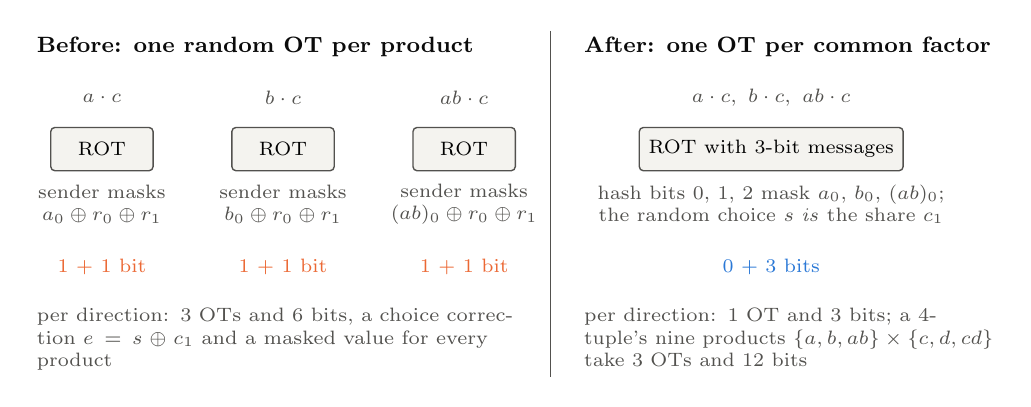
\begin{tikzpicture}[x=1cm, y=1cm]
  \tikzset{ot/.style={draw=inkTwo, line width=0.5pt, rounded corners=1.5pt, fill=boxfill, minimum width=1.3cm,
      minimum height=0.55cm, font=\scriptsize, align=center},
    bits/.style={font=\scriptsize, text=inkTwo, align=center}}
  % ---- before: three OTs per direction, one per product x*c
  \node[font=\footnotesize\bfseries, text=inkOne, anchor=west] at (-0.3,3.0) {Before: one random OT per product};
  \foreach \x/\p/\q in {0/a/a_0, 2.3/b/b_0, 4.6/ab/(ab)_0} {
    \node[bits] at (\x+0.65,2.35) {$\p\cdot c$};
    \node[ot] (o\p) at (\x+0.65,1.7) {ROT};
    \node[bits] at (\x+0.65,1.0) {sender masks\\$\q \oplus r_0 \oplus r_1$};
    \node[font=\scriptsize, text=sTwo] at (\x+0.65,0.2) {1 + 1 bit};
  }
  \node[bits, anchor=north west, align=left, text width=6.1cm] at (-0.3,-0.2)
    {per direction: 3 OTs and 6 bits, a choice correction $e = s \oplus c_1$ and a masked value for every product};
  \draw[inkTwo, line width=0.4pt] (6.35,3.2) -- (6.35,-1.2);
  % ---- after: one OT per direction for all three products
  \begin{scope}[xshift=6.85cm]
    \node[font=\footnotesize\bfseries, text=inkOne, anchor=west] at (-0.2,3.0) {After: one OT per common factor};
    \node[bits] at (2.3,2.35) {$a\cdot c,\ b\cdot c,\ ab\cdot c$};
    \node[ot, minimum width=3.2cm] (one) at (2.3,1.7) {ROT with 3-bit messages};
    \node[bits] at (2.3,1.0) {hash bits 0, 1, 2 mask $a_0$, $b_0$, $(ab)_0$;\\the random choice $s$ \emph{is} the share $c_1$};
    \node[font=\scriptsize, text=sOne] at (2.3,0.2) {0 + 3 bits};
    \node[bits, anchor=north west, align=left, text width=5.2cm] at (-0.2,-0.2)
      {per direction: 1 OT and 3 bits; a 4-tuple's nine products $\{a, b, ab\}\times\{c, d, cd\}$ take 3 OTs and 12 bits};
  \end{scope}
\end{tikzpicture}

  \caption{Products with a common factor share one random OT. Before, each product $x\cdot c$ took one
  random OT per direction plus two sent bits. Now one OT per direction carries all $k$ products in its $k$
  message bits, and a party whose share of $c$ is fresh takes it from the OT's random choice bit.}
  \label{fig:outer}
\end{figure}

\paragraph{Beaver 3- and 4-tuples with shared OTs.} A 3-tuple $(a,b,c,ab,ac,bc,abc)$ was generated as an
AND triple $(a,b,ab)$ plus three independent share multiplications $a\cdot c$, $b\cdot c$ and $ab\cdot c$.
Each multiplication took one random OT per direction: the receiver sent a choice correction
$e = s\oplus x$, the sender a masked value $y\oplus r_0\oplus r_1$. The three products share the factor $c$.
A random OT's messages are hashes of 128-bit blocks, so one OT can carry $k$ message bits for the price of one
(\texttt{send/recv\_rot\_bitplanes}). \texttt{cot\_outer\_multiply} computes all $x_p\cdot y$ for
$k$ values $x_p$ from one OT per direction, sending $k$ masked bits and at most one correction bit.
Because $c$ is fresh, each party takes its share of $c$ from the random choice bits of its receiving OTs and
sends no correction at all (\cref{fig:outer}). A 4-tuple needs the nine products $\{a,b,ab\}\times\{c,d,cd\}$:
three OTs per direction instead of nine. Per tuple, AND triples included, a 3-tuple now needs 4 random OTs instead of 8 and a 4-tuple 10 instead of 22.
In a multi-batch PPA4 run the tuple phases fall from 19.0 to 9.2\s per process and their traffic by
43--46\% (\cref{fig:tuples}). The party-local variant used by reshare+sim, where P0 holds $b$ and P1 holds
$c$ in full, is covered by the same code with one correction bit for P0's zero share. Unit tests check all
products; ReLU exactness tests report 0 wrong outputs.

\begin{figure}[t]
  \centering% Per process, multi-batch PPA4 (24 x DATTYPE 256), flare / polynize: tuple phases before (ConvTriple e3fc972) and after (ed4f83f)
\pgfplotstableread{
x kind oldMB newMB olds news oldOT newOT
0 {3-tuples} 40.16 21.51 7.62 4.56 8 4
1 {4-tuples} 66.72 37.78 11.42 4.64 22 10
}\tuples
\begin{tikzpicture}
\begin{groupplot}[
  group style={group size=3 by 1, horizontal sep=14mm},
  paper, width=4.6cm, height=4.4cm,
  xtick=data, xticklabels from table={\tuples}{kind}, xmin=-0.6, xmax=1.6,
  ymin=0, ymajorgrids, axis x line*=bottom, axis y line*=left,
  nodes near coords, every node near coord/.style={font=\scriptsize, text=inkTwo},
]
\nextgroupplot[title={random OTs per tuple}, ymax=26, ybar=1pt, bar width=11pt]
  \addplot[fill=sOther, draw=white] table[x=x, y=oldOT] {\tuples};
  \addplot[fill=sOne, draw=white] table[x=x, y=newOT] {\tuples};
\nextgroupplot[title={P0 sent per process (MB)}, ymax=80, ybar=1pt, bar width=11pt]
  \addplot[fill=sOther, draw=white] table[x=x, y=oldMB] {\tuples};
  \addplot[fill=sOne, draw=white] table[x=x, y=newMB] {\tuples};
\nextgroupplot[title={generation time (s)}, ymax=13.5, ybar=1pt, bar width=11pt,
  legend style={at={(1.02,0.98)}, anchor=north west}]
  \addplot[fill=sOther, draw=white] table[x=x, y=olds] {\tuples};
  \addplot[fill=sOne, draw=white] table[x=x, y=news] {\tuples};
  \legend{one OT per product, one OT per common factor}
\end{groupplot}
\end{tikzpicture}

  \caption{Beaver tuple generation per process in a multi-batch PPA4 run (flare / polynize, 24 processes).}
  \label{fig:tuples}
\end{figure}

% ------------------------------------------------------------------------------------------------
\section{Online phase}\label{sec:online}

On a 0.3\ms LAN, the online phase is bound by round latency and per-round work, not by bandwidth.
Activations send about 180\,MB per ImageNet inference, 0.06\s at 25\,Gbit/s. \Cref{fig:online}
shows the steps for one ImageNet image.

\begin{figure}[t]
  \centering\pgfplotstableread{
i lo hi txt label
0 2.43 4.32 {2.43--4.32} {s10 build (baseline)}
1 1.91 2.19 {1.91--2.19} {+ TCP\_NODELAY on hpmpc's sockets}
2 1.19 1.37 {1.19--1.37} {+ pooled GEMM threads, CUT\_FRACTIONAL\_BITS\_OPT}
3 1.09 1.09 1.09 {+ lock-free pool, parallel im2col, bit scatter}
4 0.99 0.99 0.99 {+ threaded ReLU levels (adder, A2B, bit injection)}
5 0.84 0.84 0.84 {+ bulk random words, parallel adder construction}
6 0.80 0.80 0.80 {+ GEMM completion on threads}
7 0.76 0.76 0.76 {+ GEMM mask-and-send on threads}
8 0.70 0.70 0.70 {+ own PRNG stream produced ahead (RNG\_AHEAD)}
}\onlinesteps
\begin{tikzpicture}
\begin{axis}[
  paper, width=0.5\linewidth, height=6.2cm, y dir=reverse, ymin=-0.6, ymax=8.6,
  ytick=data, yticklabels from table={\onlinesteps}{label},
  xmin=0, xmax=4.6, xlabel={online time, one ImageNet image (s)},
  xmajorgrids, axis x line*=bottom, axis y line*=left,
]
  \addplot[only marks, mark=*, mark size=2pt, draw=white, fill=sOne,
    error bars/.cd, x dir=both, x explicit, error bar style={draw=sOne, line width=1pt},
    error mark options={rotate=90, mark size=2.5pt, draw=sOne}]
    table[x expr={(\thisrow{lo}+\thisrow{hi})/2}, y=i, x error minus expr={(\thisrow{hi}-\thisrow{lo})/2},
      x error plus expr={(\thisrow{hi}-\thisrow{lo})/2}] {\onlinesteps};
  \addplot[only marks, mark=none, nodes near coords, point meta=explicit symbolic,
    every node near coord/.style={font=\scriptsize, text=inkTwo, anchor=west, xshift=4pt}]
    table[x=hi, y=i, meta=txt] {\onlinesteps};
\end{axis}
\end{tikzpicture}

  \caption{Online phase of one ImageNet image on flare / polynize (ranges over runs where they varied).
  Output hashes are unchanged by every step.}
  \label{fig:online}
\end{figure}

\paragraph{Nagle, buffers and GEMM threads.} With Nagle's algorithm, a round's last small message waited for a delayed
ACK. ReLU layers were bimodal (6 or 46\ms), and the online phase varied between 2.4 and 4.3\s. With
\flag{TCP_NODELAY} it takes 1.9--2.2\s. Send and receive buffers of 100\,000 words mean fewer messages
and thread hand-offs per round. The threaded GEMM first sent its outputs in linear order while
the completion visits $64\times64$ tiles; CIFAR-10 accuracy was 0\% until both used the tile order. Its threads now live in a
lock-free pool.

\begin{figure}[t]
  \centering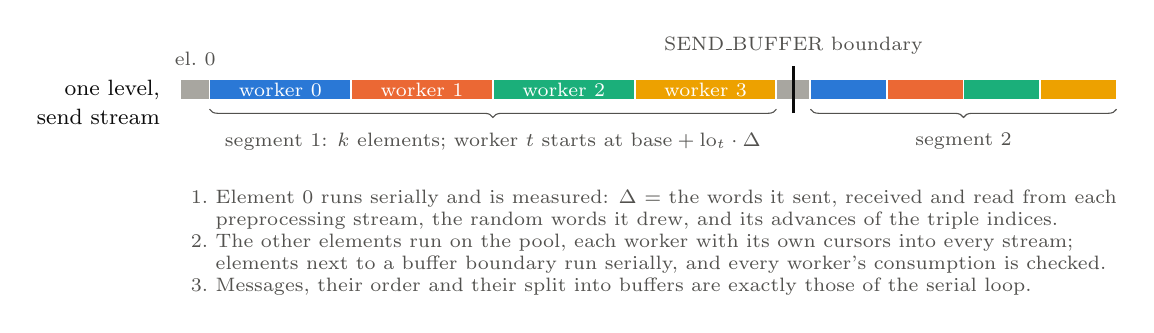
\begin{tikzpicture}[x=0.36cm, y=0.5cm]
  \node[anchor=east, font=\footnotesize, text=inkOne] at (-0.4,0) {one level,};
  \node[anchor=east, font=\footnotesize, text=inkOne] at (-0.4,-0.7) {send stream};
  % element 0, measured serially
  \fill[sOther] (0,-0.25) rectangle (1,0.25);
  \node[note, anchor=south] at (0.5,0.35) {el.\ 0};
  % segment 1 on T = 4 workers
  \foreach \t/\c in {0/sOne, 1/sTwo, 2/sThree, 3/sFour} {
    \fill[\c] (1+\t*5,-0.25) rectangle (1+\t*5+5,0.25);
    \node[font=\scriptsize, text=white] at (3.5+\t*5,0) {worker \t};
  }
  % elements near the buffer boundary run serially
  \fill[sOther] (21,-0.25) rectangle (22.2,0.25);
  % segment 2
  \foreach \t/\c in {0/sOne, 1/sTwo, 2/sThree, 3/sFour} {
    \fill[\c] (22.2+\t*2.7,-0.25) rectangle (22.2+\t*2.7+2.7,0.25);
  }
  \foreach \x in {1,6,11,16,21,22.2,24.9,27.6,30.3,33} { \draw[white, line width=0.7pt] (\x,-0.25) -- (\x,0.25); }
  \draw[inkOne, line width=1.1pt] (21.6,-0.6) -- (21.6,0.6);
  \node[note, anchor=south] at (21.6,0.65) {SEND\_BUFFER boundary};
  % braces
  \draw[decorate, decoration={brace, amplitude=3pt, mirror}, draw=inkTwo] (1,-0.5) -- (21,-0.5);
  \node[note, anchor=north] at (11,-0.85) {segment 1: $k$ elements; worker $t$ starts at $\mathrm{base} + \mathrm{lo}_t\cdot\Delta$};
  \draw[decorate, decoration={brace, amplitude=3pt, mirror}, draw=inkTwo] (22.2,-0.5) -- (33,-0.5);
  \node[note, anchor=north] at (27.6,-0.85) {segment 2};
  % steps
  \node[note, anchor=north west, align=left] at (0,-2.3)
    {1.\ Element 0 runs serially and is measured: $\Delta$ = the words it sent, received and read from each\\
     \phantom{1.\ }preprocessing stream, the random words it drew, and its advances of the triple indices.\\
     2.\ The other elements run on the pool, each worker with its own cursors into every stream;\\
     \phantom{2.\ }elements next to a buffer boundary run serially, and every worker's consumption is checked.\\
     3.\ Messages, their order and their split into buffers are exactly those of the serial loop.};
\end{tikzpicture}

  \caption{\texttt{stream\_parallel\_for}: element-parallel circuit levels at batch size one. One element
  is measured; the level's remaining elements run on the worker pool with per-worker cursors into every
  stream, split at buffer boundaries.}
  \label{fig:stream}
\end{figure}

\paragraph{Element-parallel levels at batch size one.} HPMPC vectorizes only across independent inputs,
so a single image evaluated every level of a ReLU (adder steps, A2B, bit injection) element by
element on one thread. Within a level, every element runs the same code and consumes the same number of
words from each stream: sends, receives, preprocessed values, its own random words and the indices into
the triple buffers. \texttt{stream\_parallel\_for} measures this consumption on the first element and runs
the rest on the worker pool, each worker with cursors at exactly the stream positions the serial loop
would use (\cref{fig:stream}). Segments end at send/receive buffer boundaries, and a misuse check verifies
every worker's consumption. The messages, their order and all values are those of the serial loop.
With bulk random words, parallel adder construction and the GEMM mask-and-send and completion on the same
pool, the ImageNet ReLU time falls from 630 to 300\ms and the online phase from 1.09 to 0.70\s.
\flag{RNG_AHEAD} moves the party's own sequential AES stream to a background thread.

\paragraph{Rounds per ReLU.} What remains is round latency: 1,752 rounds for CIFAR-10 with RCA against 776
with PPA and 625 with PPA4 (\cref{tab:cut}). \flag{CUT_FRACTIONAL_BITS_OPT} removes the fractional bits
from the MSB adder by substituting identity elements and public constants. RCA loses 245 of its 1,997
rounds (12\%), and ReLU traffic falls 8--11\% for every adder. Preprocessing and accuracy do not change
measurably (1,134 vs.\ 1,138 of 1,752 evaluations correct with and without CUT).

\begin{table}[t]
\centering\small
\begin{tabular}{@{}lrrrrrr@{}}
\toprule
& \multicolumn{2}{c}{rounds} & \multicolumn{2}{c}{ReLU traffic (MB)} & \multicolumn{2}{c}{online (s)}\\
single batch, unfused BN & CUT & no CUT & CUT & no CUT & CUT & no CUT\\
\midrule
RCA  & 1,752 & 1,997 & 20.8 & 23.3 & 0.52 & 0.48\\
PPA  & 776 & 789 & 32.6 & 36.8 & 0.44 & 0.49\\
PPA4 & 625 & 625 & 20.1 & 21.8 & 0.42 & 0.42\\
\bottomrule
\end{tabular}
\caption{Online rounds, P0's ReLU traffic and online time for 10 CIFAR-10 images on flare / polynize,
with and without \flag{CUT_FRACTIONAL_BITS_OPT}. The time differences are within run-to-run noise.}
\label{tab:cut}
\end{table}

% ------------------------------------------------------------------------------------------------
\section{Multi-batch}\label{sec:multi}

With 24 processes of 256-bit lanes, preprocessing dominates. With more than one HE/OT thread per process,
the processes shared connections: channel $i$ used port $\mathit{base} + i\cdot\mathit{PROCESS\_NUM}$ while
process bases stepped by 3, which caused hangs and wrong triples. With a stride of $3\cdot\mathit{PROCESS\_NUM}$, preprocessing falls from
25.0 to 14.0\s with three threads per process (\cref{tab:multi}). One extra online thread per process cuts
the online phase from 0.81 to 0.67\s with an identical output hash.

\begin{table}[t]
\centering\small
\begin{tabular}{@{}rrrrrr@{}}
\toprule
HE/OT threads & preprocessing (s) & conv (s) & AND triples (s) & BN (s) & online (s)\\
\midrule
1 & 25.0 & 16.5 & 3.6 & 2.1 & 0.63\\
2 & 17.0 & 10.2 & 3.3 & 1.4 & 0.68\\
3 & 14.0 & 8.8 & 3.0 & 1.2 & 0.75\\
4 & 14.0 & 7.8 & 3.8 & 1.0 & 0.69\\
\bottomrule
\end{tabular}
\caption{Multi-batch CIFAR-10 (24 processes, 192 images, RCA, unfused BN) on flare / polynize, by HE/OT
threads per process, after the port-stride fix.}
\label{tab:multi}
\end{table}

% ------------------------------------------------------------------------------------------------
\section{Correctness and reproducibility}\label{sec:correct}

Fast code is only useful if its outputs are right and repeatable. We made every run bit-reproducible and
compared each threaded build against a serial one; this exposed the following bugs.

\begin{itemize}\itemsep1pt
\item \textbf{Nondeterministic OT.} COT and multiplexer triple shares are the ferret outputs, and hpmpc
  truncates shares locally, so their per-run randomness changed the outputs. ConvTriple's PRGs are now seeded per party, stage, call and
  task, and a scoped override seeds emp's default PRGs per OT pack and worker (\texttt{DetSeedScope}).
\item \textbf{Worker race in P0's A2B.} For the reshare+sim skip with PPA4, P0 chooses each group's slice
  masks from the Beaver 3-tuples that the group's adder will consume, found through a count of groups prepared so far. On
  the worker pool that count was one shared global. Threaded PPA4 reshare+sim with fused BN gave a different
  output every run. The count is now a per-worker stream index. The race stayed hidden whenever the pool threads woke one after another.
\item \textbf{Hangs.} A lost wake-up at connection start, where flag and broadcast were not under the waiters' mutex, and a stale listener
  into whose backlog the next phase's peer connected.
\item \textbf{Multi-batch a2b.} The A2B mask bake derived the conv mask by casting transposed words to lanes,
  which holds only for 32-bit lanes; with 256-bit registers the a2b families classified 13--29 of 192
  images. The mask is now computed value by value with the A2B's own inverse packing, which leaves single-batch
  hashes unchanged, and the multi-batch a2b families classify 99--132 of 192 images, like the plain family.
\item \textbf{Public weights with unfused BN.} With public weights the first convolution's output is
  still the data owner's sharing (the other party's mask is zero), and SecureML truncation of that sharing wraps for positive values:
  0 of 10 correct. The owner now truncates it exactly and re-masks, in the same single message.
\item \textbf{Test harness.} The ReLU tests fed unbaked inputs to the reshare+sim skip (35\% wrong); the
  harness now declares its inputs unbaked.
\end{itemize}

After these fixes, all 60 threaded variants (30 single-batch, 30 multi-batch) reproduce their serial build's output hash on flare /
polynize, and repeated runs are bit-identical. Hashes differ between the machine pairs, because the PRNG
draws 512-bit AES blocks with VAES-512 on Zen~4 and 256-bit blocks on Zen~3.

% ------------------------------------------------------------------------------------------------
\section{Evaluation of all variants}\label{sec:eval}

\begin{figure}[p]
  \centering\begin{tikzpicture}
\begin{groupplot}[
  group style={group size=4 by 1, horizontal sep=2.5mm, yticklabels at=edge left},
  paper, height=12.2cm, width=4.15cm, y dir=reverse, ymin=-0.8, ymax=33.6,
  ytick=data, yticklabels from table={data/matrix_s.dat}{variant},
  xmajorgrids, axis x line*=bottom, axis y line*=left, enlarge x limits=0.06,
  title style={align=center},
]
\nextgroupplot[title={single batch\\preprocessing (s)}, xmin=1.0, xmax=3.4]
  \addplot[dotfp] table[x=prefp, y=x] {data/matrix_s.dat};
  \addplot[dotag] table[x=preag, y=x] {data/matrix_s.dat};
  \draw[gridc, line width=0.6pt] (axis cs:1.4,16.4) -- (axis cs:3.6,16.4);
\nextgroupplot[title={single batch\\online (s)}, xmin=0.28, xmax=0.62]
  \addplot[dotfp] table[x=onfp, y=x] {data/matrix_s.dat};
  \addplot[dotag] table[x=onag, y=x] {data/matrix_s.dat};
  \draw[gridc, line width=0.6pt] (axis cs:0.28,16.4) -- (axis cs:0.62,16.4);
\nextgroupplot[title={multi-batch\\preprocessing (s)}, xmin=6, xmax=30,
  legend style={at={(0.0,-0.045)}, anchor=north, legend columns=2}]
  \addplot[dotfp] table[x=prefp, y=x] {data/matrix_m.dat};
  \addplot[dotag] table[x=preag, y=x] {data/matrix_m.dat};
  \legend{flare / polynize (Zen 4), algofi / goracle (Zen 3)}
  \draw[gridc, line width=0.6pt] (axis cs:10,16.4) -- (axis cs:38,16.4);
\nextgroupplot[title={multi-batch\\online (s)}, xmin=0.45, xmax=1.2]
  \addplot[dotfp] table[x=onfp, y=x] {data/matrix_m.dat};
  \addplot[dotag] table[x=onag, y=x] {data/matrix_m.dat};
  \draw[gridc, line width=0.6pt] (axis cs:0.45,16.4) -- (axis cs:1.2,16.4);
\end{groupplot}
\end{tikzpicture}

  \caption{All 30 variants, CIFAR-10 ResNet50 (final builds). Upper block: fused BN; lower block: unfused BN.
  Single batch: 10 images, median of two runs. Multi-batch: 192 images, 24 processes. Tables with every value:
  \texttt{docs/VARIANT\_PERFORMANCE.md}.}
  \label{fig:matrix}
\end{figure}

\Cref{fig:matrix} shows preprocessing and online time for every variant on both machine pairs.

\paragraph{Single batch.} On flare / polynize, preprocessing takes 1.6--2.2\s with RCA,
2.3--2.5\s with PPA and 2.5--2.8\s with PPA4 when BN is fused, and 1.9--2.4, 2.6--2.9 and 2.7--3.1\s
unfused; the a2b families sit at the upper end. The online phase takes 0.35--0.52\s. Because it is
round-latency-bound, PPA and PPA4 are slightly faster online than RCA despite more AND gates. The fastest
configuration in total is RCA with fused BN (1.66\s + 0.40\s).

\paragraph{Multi-batch.} 192 images take 12.5--16.6\s (RCA), 15.7--19.8\s (PPA) and 18.7--24.4\s (PPA4)
of preprocessing and 0.54--0.79\s online. Per image that is 65--127\ms of preprocessing, against 166--310\ms in single batch.

\paragraph{Machines.} In single batch, algofi / goracle is 1--16\% slower in preprocessing than flare / polynize and
about equal online. Multi-batch is compute-bound, and there Zen~3 needs 1.4--1.7$\times$ as long:
it lacks AVX-512 for the HE NTTs and the GEMM.

\begin{figure}[t]
  \centering% Round 2 -> round 4 (shared-OT tuples, batched BN) -> final (concurrent conv triples; multi-batch lanes),
% plain family, flare / polynize. Data: data/rounds_{s,m}.dat from make_data.py
\begin{tikzpicture}
\begin{groupplot}[
  group style={group size=2 by 1, horizontal sep=6mm, yticklabels at=edge left},
  paper, width=5.6cm, height=4.6cm, y dir=reverse, ymin=-0.6, ymax=5.6,
  ytick=data, yticklabels from table={data/rounds_s.dat}{label},
  xmajorgrids, axis x line*=bottom, axis y line*=left,
]
\nextgroupplot[title={single batch, 10 images (s)}, xmin=1.0, xmax=4.6]
  \addplot[forget plot, only marks, mark=none, error bars/.cd, x dir=both, x explicit, error mark=none,
    error bar style={draw=inkTwo!45, line width=1.6pt}]
    table[x=fin, y=i, x error plus expr={max(\thisrow{r2}-\thisrow{fin},0)}, x error minus expr={0}] {data/rounds_s.dat};
  \addplot[only marks, mark=*, mark size=2pt, fill=sOther, draw=white] table[x=r2, y=i] {data/rounds_s.dat};
  \addplot[only marks, mark=*, mark size=2pt, fill=sTwo, draw=white] table[x=r4, y=i] {data/rounds_s.dat};
  \addplot[only marks, mark=*, mark size=2pt, fill=sOne, draw=white] table[x=fin, y=i] {data/rounds_s.dat};
\nextgroupplot[title={multi-batch, 192 images (s)}, xmin=6, xmax=33,
  legend style={at={(1.02,0.98)}, anchor=north west}]
  \addplot[forget plot, only marks, mark=none, error bars/.cd, x dir=both, x explicit, error mark=none,
    error bar style={draw=inkTwo!45, line width=1.6pt}]
    table[x=fin, y=i, x error plus expr={max(\thisrow{r2}-\thisrow{fin},0)}, x error minus expr={0}] {data/rounds_m.dat};
  \addplot[only marks, mark=*, mark size=2pt, fill=sOther, draw=white] table[x=r2, y=i] {data/rounds_m.dat};
  \addplot[only marks, mark=*, mark size=2pt, fill=sTwo, draw=white] table[x=r4, y=i] {data/rounds_m.dat};
  \addplot[only marks, mark=*, mark size=2pt, fill=sOne, draw=white] table[x=fin, y=i] {data/rounds_m.dat};
  \legend{round 2, round 4, final}
\end{groupplot}
\end{tikzpicture}

  \caption{Preprocessing of the plain family before (round 2) and after (round 4) the shared-OT tuples and the
  batched BN triples (flare / polynize).}
  \label{fig:r2r4}
\end{figure}

\paragraph{The last two optimizations.} \Cref{fig:r2r4} isolates the effect of the shared-OT tuples and the batched BN
triples. PPA4 gains most: single batch $4.35\to2.68\s$ unfused and $3.46\to2.61\s$ fused, multi-batch
$31.5\to22.6\s$ and $30.2\to20.2\s$. Unfused RCA gains $2.51\to1.94\s$ from the batched BN.

\subsection{Fully shared masks and public weights}\label{sec:kpw}

Two further settings change who holds the weights. With \flag{A_KNOWN=0} both parties hold shares of
the weight masks as well as of the activation masks, so the conv, FC and BN triples are AB triples for
which both parties encrypt. With public weights (\flag{PUBLIC_WEIGHTS=1}) the linear layers multiply locally
and need no triples at all. We run public weights with \flag{TRUNC_DELAYED=1} and
\flag{BIT_INJECTION_TRUNC_SIM=1}: each linear layer's truncation is deferred and folded into the next
ReLU's bit injection instead of costing a round of its own. \Cref{fig:settings} compares both settings
with the secret-weight default for the plain family.

\begin{figure}[t]
  \centering\begin{tikzpicture}
\begin{groupplot}[
  group style={group size=4 by 1, horizontal sep=6mm, yticklabels at=edge left, group name=set},
  paper, height=4.7cm, width=3.95cm, y dir=reverse, ymin=-0.6, ymax=5.6,
  ytick=data, yticklabels from table={data/settings_s.dat}{label},
  xmajorgrids, axis x line*=bottom, axis y line*=left, title style={align=center},
  unbounded coords=discard,
]
\nextgroupplot[title={single batch\\preprocessing (s)}, xmin=0.6, xmax=3.0]
  \addplot[dotfp] table[x=pre1, y=y] {data/settings_s.dat};
  \addplot[dotag] table[x=pre0, y=y] {data/settings_s.dat};
  \addplot[only marks, mark=square*, mark size=1.8pt, draw=white, line width=0.5pt, fill=sThree] table[x=prepw, y=y] {data/settings_s.dat};
\nextgroupplot[title={single batch\\online (s)}, xmin=0.2, xmax=0.6]
  \addplot[dotfp] table[x=on1, y=y] {data/settings_s.dat};
  \addplot[dotag] table[x=on0, y=y] {data/settings_s.dat};
  \addplot[only marks, mark=square*, mark size=1.8pt, draw=white, line width=0.5pt, fill=sThree] table[x=onpw, y=y] {data/settings_s.dat};
\nextgroupplot[title={multi-batch\\preprocessing (s)}, xmin=0, xmax=26,
  legend to name=setlegend, legend columns=3, legend style={column sep=8pt}]
  \addplot[dotfp] table[x=pre1, y=y] {data/settings_m.dat};
  \addplot[dotag] table[x=pre0, y=y] {data/settings_m.dat};
  \addplot[only marks, mark=square*, mark size=1.8pt, draw=white, line width=0.5pt, fill=sThree] table[x=prepw, y=y] {data/settings_m.dat};
  \legend{{secret weights, \flag{A_KNOWN=1}}, {secret weights, \flag{A_KNOWN=0}}, {public weights}}
\nextgroupplot[title={multi-batch\\online (s)}, xmin=0.2, xmax=1.0]
  \addplot[dotfp] table[x=on1, y=y] {data/settings_m.dat};
  \addplot[dotag] table[x=on0, y=y] {data/settings_m.dat};
  \addplot[only marks, mark=square*, mark size=1.8pt, draw=white, line width=0.5pt, fill=sThree] table[x=onpw, y=y] {data/settings_m.dat};
\end{groupplot}
\node[anchor=north] at ($(set c1r1.south west)!0.5!(set c4r1.south east) + (0,-0.75cm)$) {\pgfplotslegendfromname{setlegend}};
\end{tikzpicture}

  \caption{Secret weights with \flag{A_KNOWN=1} (default) and \flag{A_KNOWN=0}, and public weights, plain family,
  flare / polynize. Runtime does not depend on the values, so the \flag{A_KNOWN=0} times are valid although
  its accuracy is not.}
  \label{fig:settings}
\end{figure}

\paragraph{Public weights.} Only the ReLU material remains to be preprocessed: across all 30 variants,
preprocessing takes 0.92--2.03\s per 10 images and 3.5--14.3\s per 192 images, 27--53\% and 38--75\%
less than the same variant with secret weights. The online phase takes 0.27--0.41\s and 0.33--0.42\s
(5--29\% and 29--50\% less): convolutions send nothing, and the truncation shares the bit injection's message. With the AdamW model, the public-weight variants
classify 63--73 of 100 images in single batch and 115--131 of 192 (60--68\%) in multi-batch. Unfused
BatchNorm needed the first-layer truncation fix of \cref{sec:correct}; before it, those variants classified 0 of 10 images.

\paragraph{Fully shared masks.} With \flag{A_KNOWN=0} the linear-layer triples are AB triples, and preprocessing
traffic grows by a factor of 1.4--1.9 (for RCA, unfused BN, 10 images: 229 to 428\,MB). In single batch the preprocessing
is nevertheless 3--18\% faster (1.50--2.83\s over the 30 variants): both parties encrypt, and the pipelined convolutions
keep both of them busy (conv phase 0.65 to 0.48\s). In multi-batch, with three threads per process, it is
3--16\% slower (13.8--26.4\s). The online phase takes 0.34--0.52\s and 0.56--0.73\s. The accuracy, however, is at chance level (0--1 of 10 in
every configuration we tried, including \flag{TRUNC_DELAYED=1} with the truncation in the bit injection).
With both masks shared, the product mask $\lambda_w\lambda_x$ is itself a full-range sharing, and the
probabilistic local truncation of the layer outputs wraps. \flag{A_KNOWN=1} avoids this because one party holds the
weight mask and the conv triple delivers its product exactly. A fix needs exact or reduced-slack truncation for
ABY2, which the protocol does not implement yet.


\subsection{Final accuracy}

\begin{figure}[t]
  \centering\begin{tikzpicture}
\begin{axis}[
  paper, width=0.62\linewidth, height=11.5cm, y dir=reverse, ymin=-0.8, ymax=33.6,
  ytick=data, yticklabels from table={data/accuracy.dat}{variant},
  xmin=50, xmax=82, xlabel={correctly classified (\%)},
  xmajorgrids, axis x line*=bottom, axis y line*=left,
  legend style={at={(0.5,-0.07)}, anchor=north, legend columns=2, column sep=6pt},
]
  \addplot[only marks, mark=*, mark size=2pt, fill=sOne, draw=white] table[x=single, y=x] {data/accuracy.dat};
  \addplot[only marks, mark=diamond*, mark size=2.4pt, fill=sTwo, draw=white] table[x=multi, y=x] {data/accuracy.dat};
    \addplot[sOne, dashed, line width=0.8pt] coordinates {(76,-0.8) (76,33.6)};
  \addplot[sTwo, dashed, line width=0.8pt] coordinates {(71.9,-0.8) (71.9,33.6)};
  \legend{{single batch, 100 images}, {multi-batch, 192 images}, {plaintext, 100 images (76\%)}, {plaintext, 192 images (71.9\%)}}
  \draw[gridc, line width=0.6pt] (axis cs:50,16.4) -- (axis cs:82,16.4);
  \node[note, anchor=east] at (axis cs:81.6,0.2) {fused BN};
  \node[note, anchor=east] at (axis cs:81.6,17.6) {unfused BN};
\end{axis}
\end{tikzpicture}

  \caption{Accuracy with the AdamW-trained ResNet50, standard probabilistic truncation. Single batch on
  flare / polynize, multi-batch on algofi / goracle (a2b families: builds with the multi-batch A2B bake).}
  \label{fig:acc}
\end{figure}

\begin{table}[t]
\centering\small
\begin{tabular}{@{}lrr@{}}
\toprule
Setting & images & correct\\
\midrule
Plaintext, float (PyTorch) & 100 / 192 & 76 / 138 (71.9\%)\\
Trio 3PC, standard configuration & 100 & 71\\
Trio 3PC, reduced-slack truncation (\flag{TRUNC_APPROACH=1}) & 100 & 70\\
2PC ABY2, single batch, all 30 variants & 100 & 62--73\\
2PC ABY2, multi-batch, all 30 variants & 192 & 116--132\\
2PC ABY2, CUT on / off (plain family, 12 runs each) & 1,752 & 1,134 / 1,138\\
\bottomrule
\end{tabular}
\caption{Final accuracy with the AdamW-trained ResNet50 on the first CIFAR-10 test images.}
\label{tab:acc}
\end{table}

Every variant stays above 60\% (\cref{fig:acc,tab:acc}). The spread between variants
(62--73 of 100) is truncation noise: the variants draw different amounts of randomness, so different
values wrap. The adders are exact, with 0 of 32,768 random ReLU inputs wrong for each adder. Fused and unfused BN are equally accurate with this model.
With the older \texttt{Cifar\_adam\_001} model, probabilistic truncation in the 32-bit ring cost 10--17
points (Trio 56\% against 73\% in plaintext; 73\% with a 64-bit ring). The AdamW model is much less sensitive to it.

% ------------------------------------------------------------------------------------------------
\FloatBarrier
\section{Limitations and open problems}

\begin{itemize}\itemsep1pt
\item \textbf{Truncation.} ABY2 has no reduced-slack or exact truncation yet; with fully shared masks
  (\flag{A_KNOWN=0}) the local truncation wraps, and ResNet50 classifies at chance (\cref{sec:kpw}).
\item \textbf{Weights known in preprocessing.} The multi-batch a2b bake still excludes
  \flag{MODELWEIGHTS_KNOWN_DURING_PREPROCESSING}, whose prescribed shares assume one word per register.
\item \textbf{Ciphertext occupancy.} At $7\times7$ feature maps, inputs are 5--19\% data and outputs
  6--24\%. Packing the sparse outputs needs automorphisms and a larger ring ($N = 8192$).
\item \textbf{OT extension.} Ferret's LPN step and the AES key schedules of the correlation-robust hash
  are now the largest CPU costs of the Boolean preprocessing; a fixed-key hash is a security decision.
\end{itemize}

\section{Conclusion}

The largest runtime gains came from doing less redundant work in the HE evaluator (packing, lazy
transforms, pipelining). The largest communication gains came from sending only information-bearing bits:
the exact wire format, full BatchNorm ciphertexts, and OTs whose message bits carry several products. In the online phase, latency rather than bandwidth
dominates, so the gains came from Nagle-free sockets, fewer rounds and parallelizing the per-round work at batch size
one. Seeded, bit-reproducible runs made every change measurable and exposed the bugs in \cref{sec:correct}.

\begin{thebibliography}{9}\small
\bibitem{aby2} A.~Patra, T.~Schneider, A.~Suresh, H.~Yalame. ABY2.0: Improved mixed-protocol secure
  two-party computation. USENIX Security 2021.
\bibitem{cheetah} Z.~Huang, W.~Lu, C.~Hong, J.~Ding. Cheetah: Lean and fast secure two-party deep neural
  network inference. USENIX Security 2022.
\bibitem{ferret} K.~Yang, C.~Weng, X.~Lan, J.~Zhang, X.~Wang. Ferret: Fast extension for correlated OT
  with small communication. ACM CCS 2020.
\end{thebibliography}
\end{document}
